% MapOSMatic - Libre Software Meeting 2012 presentation
% -*- coding: utf-8; mode: LaTeX -*-

% Copyright (C) 2010 Maxime Petazzoni <maxime.petazzoni@bulix.org>
%                    Thomas Petazzoni <thomas.petazzoni@enix.org>
% Distributed under the terms of the Creative Commons CC-by-sa 3.0

\documentclass{beamer}
\usepackage[utf8]{inputenc}
\usepackage[american]{babel}

\mode<presentation>
\usetheme{MapOSMatic}
\setbeamercovered{dynamic}

\title{MapOSMatic: city maps for the masses}
\author{Thomas {\sc Petazzoni}}
\institute{Libre Software Meeting}
\date{July 10th, 2012}

\begin{document}

%%%%%%%%%%%%%%%%%%%%%%%%%%%%%%%%%%%%%%%%%%%%%%%%%%%%%%%%%%%%%%%%%%%%%%%

\begin{frame}
  \titlepage
\end{frame}

\begin{frame}{Thomas Petazzoni}
  \begin{itemize}
  \item {\bf Embedded Linux engineer} and trainer at Free Electrons
  \item Regular contributor to the {\bf Buildroot} project, an open-source
    embedded Linux build system
  \item Contributor to the Linux {\bf kernel}
  \item Active in the free software community: founder of {\em
      Toulibre}, founder of the {\em Agenda du Libre}
  \item {\bf One of the developer of MapOSMatic}, together with
    David Decotigny, Gaël Utard, Maxime Petazzoni, David Mentré,
    Frédéric Lehobey, Étienne Loks, and many other contributors.
  \end{itemize}
\end{frame}

\begin{frame}{Agenda}
  \begin{enumerate}
  \item Original idea and goal
  \item History
  \item Current status
  \item Technical details
  \item Future
  \end{enumerate}
\end{frame}

\begin{frame}{Original idea}
  At some point in 2009...
  \vspace{1cm}
  \\
  \Large
  \begin{quote}
    ``It would be great to be able to use OpenStreetMap data to generate
    city maps such as the ones we can see in town signs and in folded
    maps.''
  \end{quote}
  \normalsize
  \vspace{1cm}
  \hfill Gilles Lamiral, OSM contributor of Bretagne, France
\end{frame}

\begin{frame}{Public city maps}
  \begin{center}
    \includegraphics[height=0.8\textheight]{public-city-map.jpg}
  \end{center}
\end{frame}

\begin{frame}{Folded maps}
  \begin{center}
    \includegraphics[height=0.8\textheight]{folded-map.jpg}
  \end{center}
\end{frame}

\begin{frame}{Goal}
  \Large
  Create an {\bf easy-to-use Web service}, in which the user inputs
  the {\bf name of a city}, and in return gets:
  \begin{enumerate}
  \item a {\bf map} of that city, overlayed by a {\bf grid}
  \item an {\bf index of streets and amenities} associated to the map
  \end{enumerate}
\end{frame}

\begin{frame}{Development model}
  \begin{itemize}
  \item The development mainly takes place during {\bf hackfests}
  \item Hackfests are gathering of 4-6 developers for 2 to 8 days,
    fully dedicated to making progress on the project
  \item Hackfests provide an excellent productivity
  \item Maintenance and minor progress (bug fixes, translation
    updates) done outside of the hackfests, as a regular open-source
    project, with mailing-list, Git repositories, etc.
  \end{itemize}
\end{frame}

\begin{frame}{Hackfest \#0}
  \begin{itemize}
  \item August 2009, Toulouse, France
  \item Six OSM contributors
  \item No knowledge of PostgreSQL, PostGIS, Mapnik, OSM data
    structure, Cairo
  \item Initial version of MapOSMatic developed and published in 5 days
    \begin{itemize}
    \item Technologies: Python, Django, Cairo, PostgreSQL, PostGIS, Mapnik
    \end{itemize}
  \item Limited to France, no support for languages other than French
    and English, very basic user interface, OSM data never updated
  \item \url{http://www.maposmatic.org}
  \end{itemize}
\end{frame}

\begin{frame}{Hackfest \#0 results}
  \begin{center}
    \includegraphics[height=0.8\textheight]{chavagne.png}
    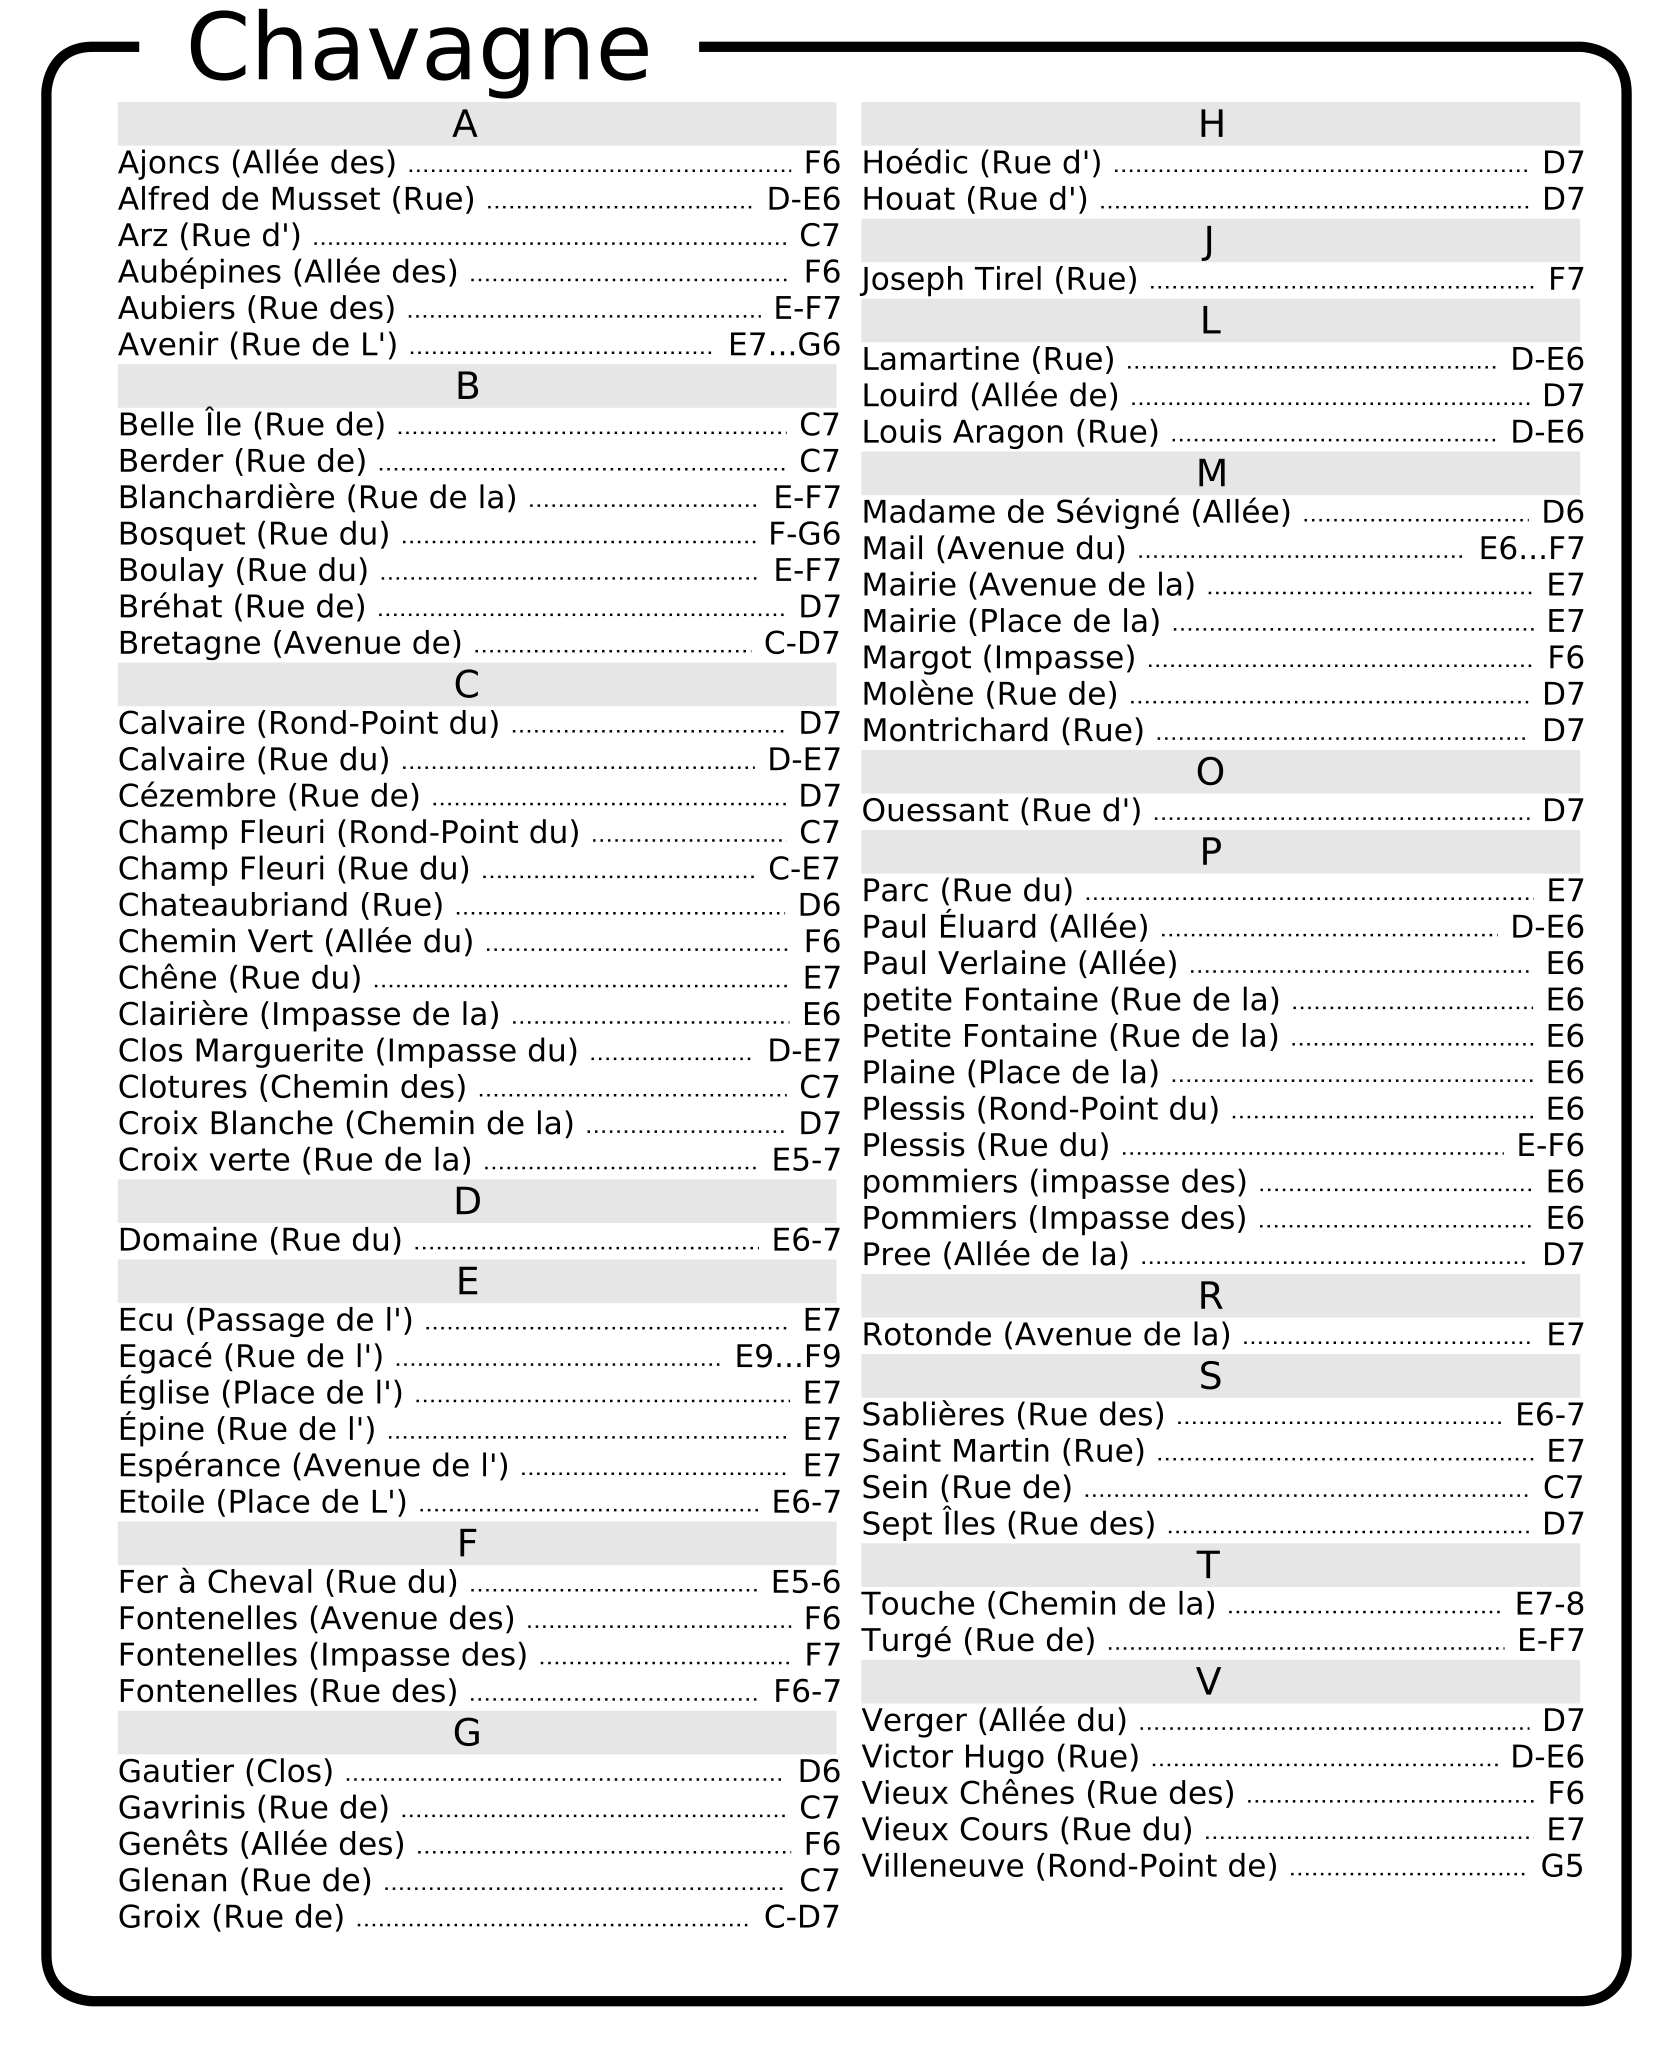
\includegraphics[height=0.8\textheight]{chavagne_index.png}
  \end{center}
\end{frame}

\begin{frame}{Hackfest \#0 map detail}

\end{frame}

\begin{frame}{Hackfest \#1}
  \begin{center}
  \end{center}
\end{frame}

\begin{frame}[t]{Conclusion}
\end{frame}

\end{document}
